\documentclass[../TDT6.tex]{subfiles}%

\begin{document}
\section{Stockage d'eau chaude}
\enonce{%
	\noindent
	\begin{minipage}[t]{.49\linewidth}
		Une masse $m = \SI{100}{\kilo\gram}$ d'eau chaude est stockée dans une cuve
		fermée de volume $V_0 = \SI{200}{L}$, que l'on modélise comme étant
		indéformable. Pour simplifier, on ne tient pas compte de l'air contenu dans
		la cuve en plus de l'eau. Suite à un échauffement accidentel, l'eau
		normalement maintenue à $T_0 = \SI{60}{\degreeCelsius}$ passe à $T =
			\SI{500}{\degreeCelsius}$.
		\smallbreak
		La vapeur d'eau est modélisée par un gaz parfait. On tient compte de la
		légère compressibilité et dilatabilité de l'eau liquide par une équation
		d'état de la forme~:
		\begin{gather*}
			\ln \frac{V}{V_0}=\alpha (T-T_0)-\chi_T(P-P_0)
			\\\beforetext{avec}
			\left\{
			\begin{aligned}
				\alpha & = \SI{3.0e-4}{K^{-1}}   \\
				\chi_T & = \SI{5.0e-10}{Pa^{-1}}
			\end{aligned}
			\right.
		\end{gather*}
		On donne le diagramme de \textsc{Clapeyron} $(P,v)$ de l'eau
		Figure~\ref{fig:stock_eau}. Plusieurs isothermes sont représentées pour des
		températures allant de 60 à \SI{600}{\degreeCelsius}. Attention, les
		échelles sont logarithmiques.
	\end{minipage}
	\hfill
	\begin{minipage}[t]{.49\linewidth}
		\vspace{0pt}
		\begin{center}
			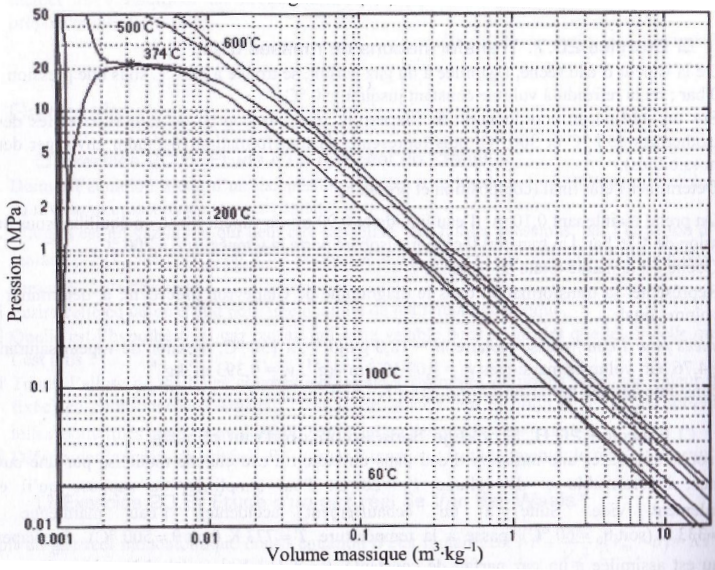
\includegraphics[width=\linewidth]{stock_eau}
			\captionof{figure}{}
			\label{fig:stock_eau}
		\end{center}
	\end{minipage}
}%

\QR{%
	Identifiez, sur le diagramme de \textsc{Clapeyron}, la courbe de rosée,
	la courbe d'ébullition, le point critique et les différentes phases dans
	lesquelles se trouve l'eau.
}{%
	\sswitch{
		\hfill
		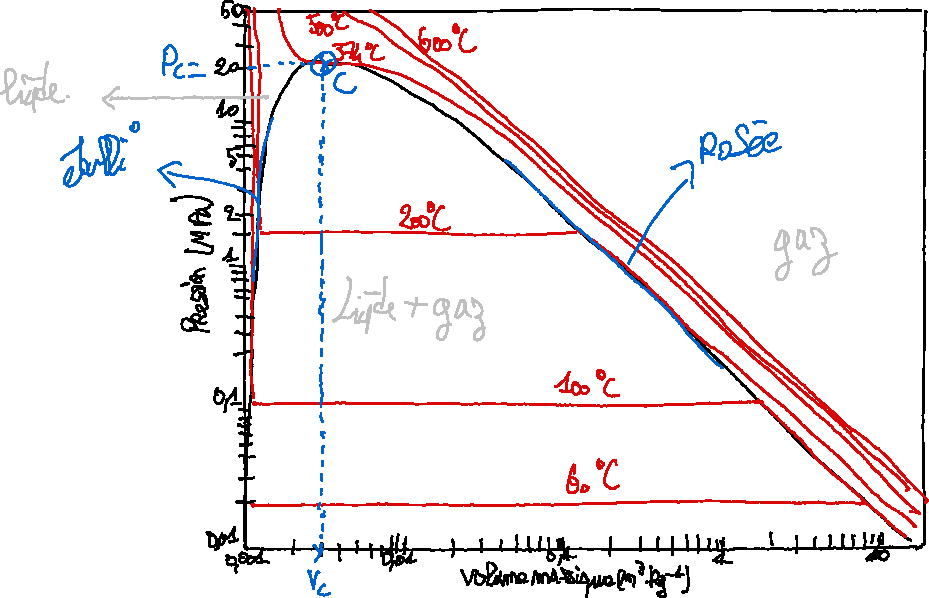
\includegraphics[width=.6\linewidth, valign=t]{stock_eau_gen}
		\hspace*{\fill}
	}{
		\leavevmode\vspace*{-15pt}\relax
		\begin{center}
			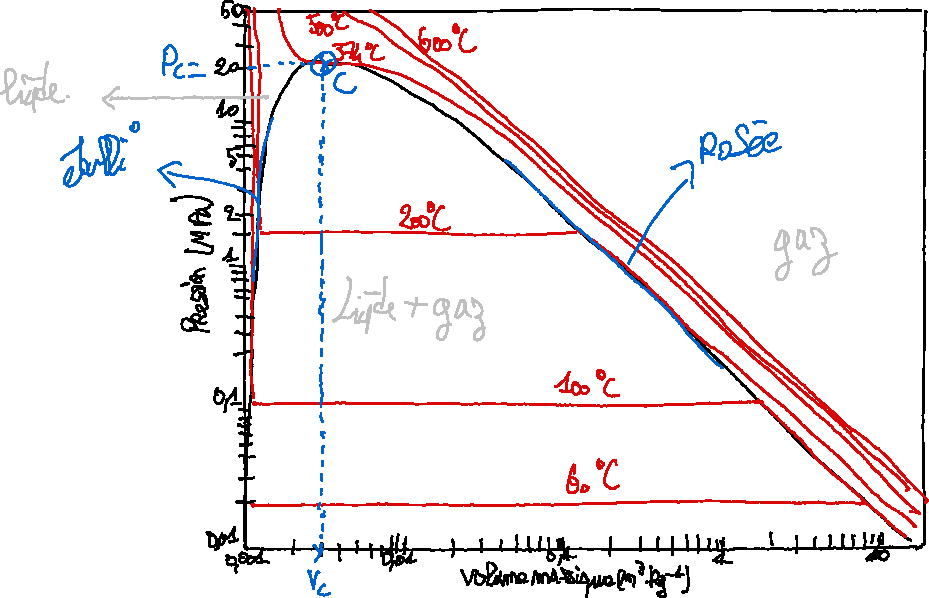
\includegraphics[width=.6\linewidth]{stock_eau_gen}
		\end{center}
	}
}%

\QR{%
Montrez que pour un équilibre liquide-vapeur, on a :
\[
	x_g = \frac{m_g}{m_g+m_{\ell}} = \frac{v-v_l}{v_g - v_{\ell}}
\]
où $m_g$ représente la masse d'eau sous la forme vapeur, $m_{\ell}$, la masse
d'eau sous forme de liquide, $v$, le volume massique du mélange, $v_g$ et
$v_{\ell}$, les volumes massiques des phases vapeur et liquide.
}{%
Soit $V_g$ et $V_{\ell}$ les volumes de gaz et de liquide, et $V = V_g +
	V_{\ell}$ le volume total.
\begin{DispWithArrows*}[]
	v &= \frac{V_g}{m} + \frac{V_{\ell}}{m}
	\Arrow{$v = V/m \Lra V = mv$}
	\\\Lra
	v &= \frac{m_gv_g}{m} + \frac{m_{\ell}v_{\ell}}{m}
	\Arrow{$x_g = m_g/m$}
	\\\Lra
	v &= x_gv_g + x_{\ell}v_{\ell}
	\Arrow{$x_g = 1-x_{\ell}$}
	\\\Lra
	v &= (1-x_{\ell})v_g + x_{\ell}v_{\ell}
	\\\Lra
	x_{\ell} = \frac{v_g-v}{v_g-v_{\ell}}
	\quad & \text{et} \quad
	x_g = \frac{v-v_{\ell}}{v_g-v_{\ell}}
	\qed
\end{DispWithArrows*}
}%

\QR{%
	En utilisant le diagramme de \textsc{Clapeyron}, déterminer la
	composition du mélange liquide-gaz initial.
}{%
	~
	\smallbreak
	\vspace{-15pt}
	\begin{isd}[righthand ratio=.35, interior hidden]
		On a $v_0 = \frac{V_0}{m}$, avec $V_0 = \SI{200}{L}$ et $m = \SI{100}{kg}$,
		soit
		\[
			v_0 = \SI{2.00e-3}{m^3.kg^{-1}}
		\]
		On est à $T = \SI{60}{\degreeCelsius}$, soit avec le graphique un
		\textbf{mélange liquide-gaz}.
		\smallbreak
		Le théorème des moments donne alors
		\begin{align*}
			x_g = \frac{AM}{AB} & = \frac{v_0-v_{\ell}}{v_g-v_{\ell}}
			\qav
			\left\{
			\begin{array}{rcl}
				v_{\ell} & = & \SI{1e-3}{m^3.kg^{-1}}
				\\
				v_0      & = & \SI{2.33e-3}{m^3.kg^{-1}}
				\\
				v_g      & = & \SI{8}{m^3.kg^{-1}}
			\end{array}
			\right.                                                   \\
			\makebox[0pt][l]{$\phantom{\AN}\xul{\phantom{x_g = \num{1.25e-4}}}$}
			\AN
			x_g                 & = \num{1.25e-4}
			\\\beforetext{D'où}
			                    &
			\left\{
			\begin{array}{ll}
				m_g      & = mx_g = \SI{13}{g}
				\\
				m_{\ell} & = m(1-x_g) \approx \SI{100}{kg}
			\end{array}
			\right.
		\end{align*}
		\tcblower
		\begin{center}
			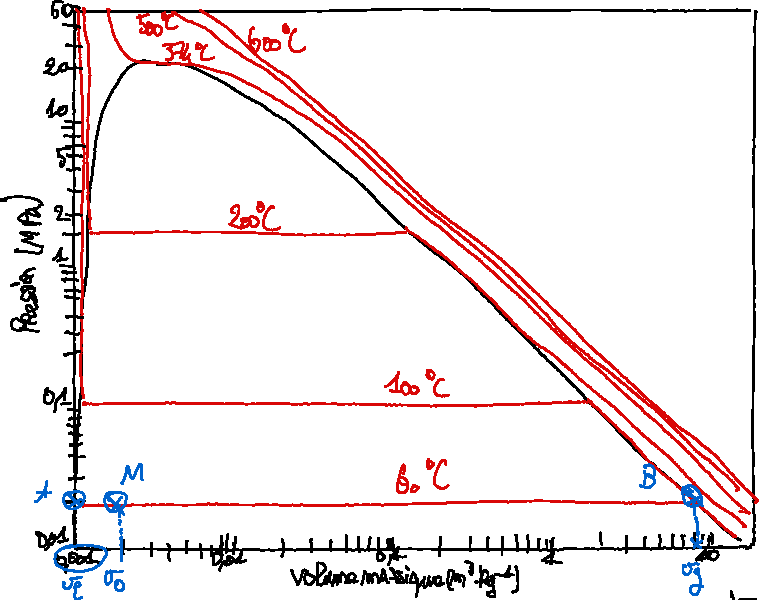
\includegraphics[width=\linewidth]{stock_eau_init}
		\end{center}
	\end{isd}
}%

\QR{%
	Sous quelle forme trouve-t-on l'eau après l'échauffement accidentel~?
	Déterminer la pression $P$ correspondante. Commenter.
}{%
	~
	\smallbreak
	\vspace{-15pt}
	\begin{isd}[righthand ratio=.4, interior hidden]
		Volume $V$ fixé et masse $m$ fixée, donc $v$ fixé~: on se déplace
		verticalement depuis $v_0$ pour atteindre l'isotherme
		$\SI{500}{\degreeCelsius}$. On est alors dans l'\textbf{état supercritique}.
		Avec $V = V_0$,
		\begin{gather*}
			\underbracket[1pt]{\ln (\frac{V}{V_0})}_{=0} = \alpha (T - T_0)-\chi_T
			(P-P_0)
			\\\Lra
			\boxed{P = P_0 + \frac{\alpha (T-T_0)}{\chi_T}}
			\\\Ra
			\xul{P = \SI{2.1e3}{bar}}
		\end{gather*}
		Il a donc \textbf{risque d'explosion}~!
		\tcblower
		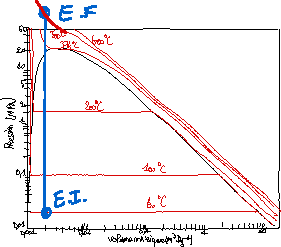
\includegraphics[width=\linewidth]{stock_eau_echauff}
	\end{isd}
}%

\QR{%
	La soupape de sécurité permet au fur et à mesure du chauffage de laisser
	de la vapeur d'eau s'échapper~: la cuve est finalement presque vide et ne
	contient plus que $m_0 = \SI{400}{g}$ d'eau. Déterminer la pression
	finale et conclure.
}{%
	~
	\smallbreak
	\vspace{-15pt}
	\begin{isd}[righthand ratio=.4, interior hidden]
		Toujours à $V_0$, mais $m_0 = \SI{400}{g}$ donc
		\[
			v_0 = \SI{0.500}{m^3.kg^{-1}}
		\]
		On est donc sur l'isotherme à $\SI{500}{\degreeCelsius}$ pour l'abscisse
		$v_0$~; on lit
		\[
			\xul{P = \SI{0.7}{MPa} = \SI{7}{bar}}
		\]
		et le système est totalement gazeux. \textbf{Il n'y a plus de risque
			d'explosion}.
		\tcblower
		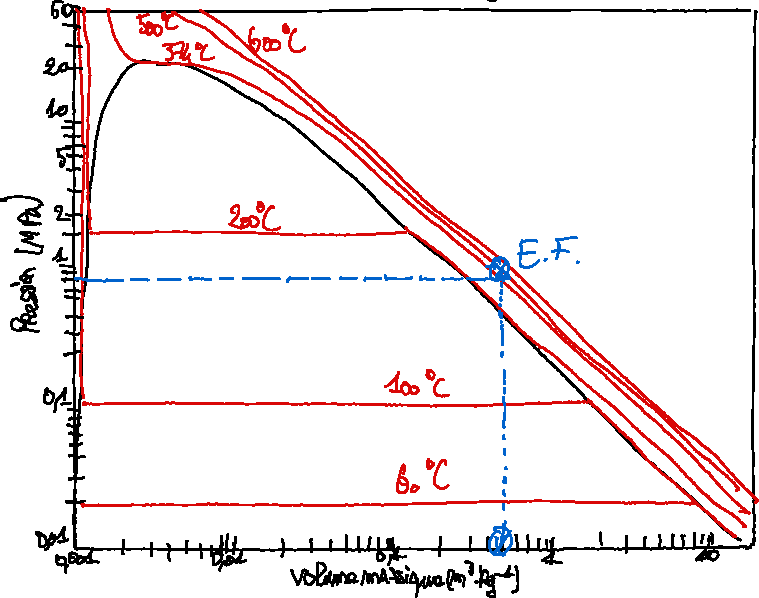
\includegraphics[width=\linewidth]{stock_eau_echauff2}
	\end{isd}
}%

\end{document}
